
\documentclass[UTF8]{ctexart}
\usepackage{amsmath}
\usepackage{graphicx}
\usepackage{ctex}
\usepackage{graphicx}
\usepackage{caption2}
\usepackage{subfigure}
\usepackage{float}
\usepackage{listings}
\usepackage{fancyhdr}
\CTEXsetup[format={\Large\bfseries}]{section}
\title{\vspace{-3cm}\textbf{\zihao{1}算法设计与分析}\\\zihao{2}(实验报告)\\\vspace{+10cm}}
\pagestyle{fancy}
\fancyhead{}
\renewcommand\headrulewidth{0pt}
\begin{document}
\date{}
\maketitle
\begin{center}
     \zihao{3} 姓名:孙清远\\班级:1904301\\ \quad\ \,学号:2190400211
\end{center}
\newpage
\section{排序}
\subsection{算法原理}
  实验一要求实现两种不同的排序算法,并使用11个大小为$10^6$的不同重复率的
  数据集测定算法的执行时间,最后与库函数进行对比。\par
  此实验选取快速排序与二分归并排序算法作为实验对象。\par
  快速排序是C.R.A.Hoare于1962年提出的一种划分交换排序。它采用了一种分治的策略,通常称其为分治法(Divide-and-ConquerMethod),
  由于排序效率在同为O(N*logN)的几种排序方法中效率较高,因此经常被采用。\par
  快速排序大致可分为以下几个步骤:
  \begin{itemize}
      \item 首先设定一个分界值,通过该分界值将数组分成左右两部分。
      \item 将大于或等于分界值的数据集中到数组右边,小于分界值的数据集中到数组的左边。此时,左边部分中各元素都小于或等于分界值,而右边部分中各元素都大于或等于分界值。
      \item 然后,左边和右边的数据可以独立排序。对于左侧的数组数据,又可以取一个分界值,将该部分数据分成左右两部分,同样在左边放置较小值,右边放置较大值。右侧的数组数据也可以做类似处理。
      \item 重复上述过程,可以看出,这是一个递归定义。通过递归将左侧部分排好序后,再递归排好右侧部分的顺序。当左、右两个部分各数据排序完成后,整个数组的排序也就完成了。
  \end{itemize}
  \par
  在第一步选取基准数的时候,数的大小决定了决定了下一步划分集合的
  均匀程度,集合划分越均匀,花费的时间越少。因此如果要优化算法,可以在选取基准数的时候
  采用随机选取的策略来降低时间复杂度。 \par
  在划分集合的过程中,通常是在数组左右设置两个游标,从右侧游标开始,找到一个小于等于基准数的数,
  左侧游标找到一个大于基准数的数,然后交换这两个数的位置,如此重复,直到这两个游标开始重合。 \par
  此时整个数组已经被划分为两个部分,这两个部分可以递归的去处理。\par
  归并排序(Merge Sort)是建立在归并操作上的一种有效,稳定的排序算法,该算法是采用分治法(Divide and Conquer)的一个非常典型的应用。将已有序的子序列合并,得到完全有序的序列;即先使每个子序列有序,再使子序列段间有序。若将两个有序表合并成一个有序表,称为二路归并。\par
  我们通常采用的是自上而下的归并排序,大致可分为三步:
  \begin{itemize}
      \item 分解 -- 将当前区间一分为二,即求分裂点 mid = (low + high)/2。
      \item 求解 -- 递归地对两个子区间a[low...mid] 和 a[mid+1...high]进行归并排序。递归的终结条件是子区间长度为1。
      \item 合并 -- 将已排序的两个子区间a[low...mid]和 a[mid+1...high]归并为一个有序的区间a[low...high]。
  \end{itemize}
  \par
  下面是两种排序算法的示意图:
  \begin{figure}[htbp]
    \centering
    \subfigure[快速排序]{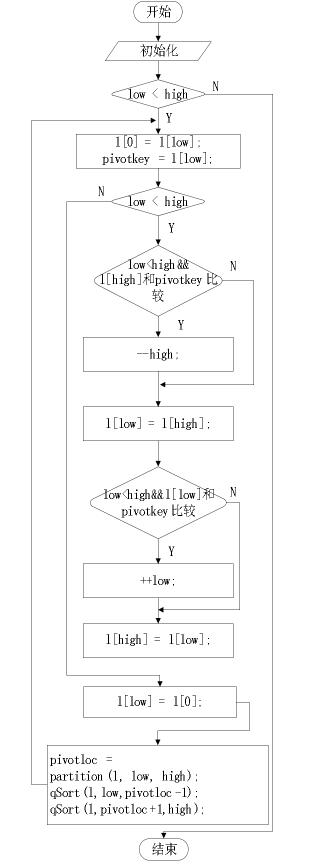
\includegraphics[width=0.3\textwidth]{quicksort.jpg}}
    \subfigure[归并排序]{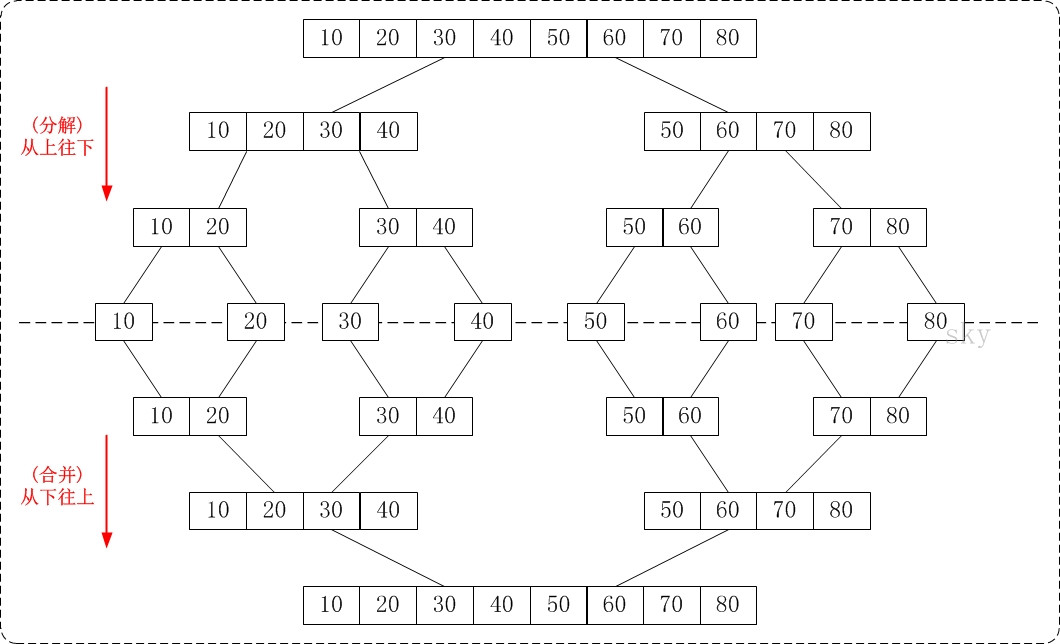
\includegraphics[height=7cm,width=0.6\textwidth]{mergesort.jpg}}
    \caption{算法图解}
    \label{fig:label1}
    \end{figure}
\subsection{算法描述}
\subsubsection{快速排序伪码描述}
算法Quicksort(A,p,r)\par
输入:数组A[p..r]\par
输出:排好序的数组A
 \begin{enumerate}
    \item if $p \gets r$
    \item then $q \gets Partition(A,p,r) $
    \item \qquad $A[p] \leftrightarrow A[q] $
    \item \qquad $Quicksort(A,p,q-1) $
    \item \qquad $Quicksort(A,q+1,r) $
\end{enumerate}
\par
初始置p=1,r=n,然后调用上述算法。\par
Partition(A,p,r)
\begin{enumerate}
    \item $x \gets A[p]$
    \item $i \gets p$
    \item $j\gets r+1 $
    \item while \ true \ do
    \item \qquad $repeat j \gets j-1 $
    \item \qquad $until A[j] \le x $
    \item \qquad $repeat i \gets i+1 $
    \item \qquad $until A[i]>x $
    \item \qquad if $i<j $
    \item \qquad then $A[i] \leftrightarrow A[j] $
    \item \qquad else return j
\end{enumerate}
\subsubsection{归并排序伪码描述}
算法MergeSort(A,p,r)\par
输入:数组A[p..r]\par
输出:元素按从小到大排序的数组A\par
\begin{enumerate}
    \item if $p<r$
    \item then $q \gets \lfloor (p+r)/2 \rfloor$
    \item \qquad MergeSort(A,p,q)
    \item \qquad MergeSort(A,q+1,r)
    \item \qquad Merge(A,p,q,r)
\end{enumerate}
\subsection{算法程序}
\subsubsection{快速排序代码描述}
\begin{lstlisting}[language=C++]
int Data[1000000 + 10];
int temp[1000000 + 10];
void quickSort(int left, int right, int* arr)
{
	if (left >= right)
		return;
	int i, j, base, temp;
	i = left, j = right;
	base = arr[left]; 
	while (i < j)
	{
		while (arr[j] >= base && i < j)
			j--;
		while (arr[i] <= base && i < j)
			i++;
		if (i < j)
		{
			temp = arr[i];
			arr[i] = arr[j];
			arr[j] = temp;
		}
	}

	arr[left] = arr[i];
	arr[i] = base;
	quickSort(left, i - 1, arr);
	quickSort(i + 1, right, arr);
}
\end{lstlisting}
\subsubsection{归并排序算法描述}
\begin{lstlisting}[language=C++]
void merge(int elem[], int lo, int hi, int mid)
{
    int i = lo, j = mid + 1;
    memset(temp, 0, sizeof(int) * 10);
    int count = 0;
    while (i <= mid && j <= hi)
    {
        if (elem[i] <= elem[j])
        {
            temp[count] = elem[i];
            count++;
            i++;
        }
        else
        {
            temp[count] = elem[j];
            count++;
            j++;
        }
    }
    while (i <= mid)
    {
        temp[count] = elem[i];
        count++;
        i++;
    }
    while (j <= hi)
    {
        temp[count] = elem[j];
        count++;
        j++;
    }
    int k, n;
    n = 0;
    for (k = lo; k <= hi; k++)
    {
        elem[k] = temp[n++];
    }
}
void MergeSort(int elem[], int lo, int hi)
{
    if (lo >= hi)return;
    else
    {
        int mid = (lo + hi) / 2;
        MergeSort(elem, lo, mid);
        MergeSort(elem, mid + 1, hi);
        merge(elem, lo, hi, mid);
    }
}
\end{lstlisting}
\subsection{实验结果}
\subsubsection{快速排序实验结果}
\begin{figure}[H]
    \centering
    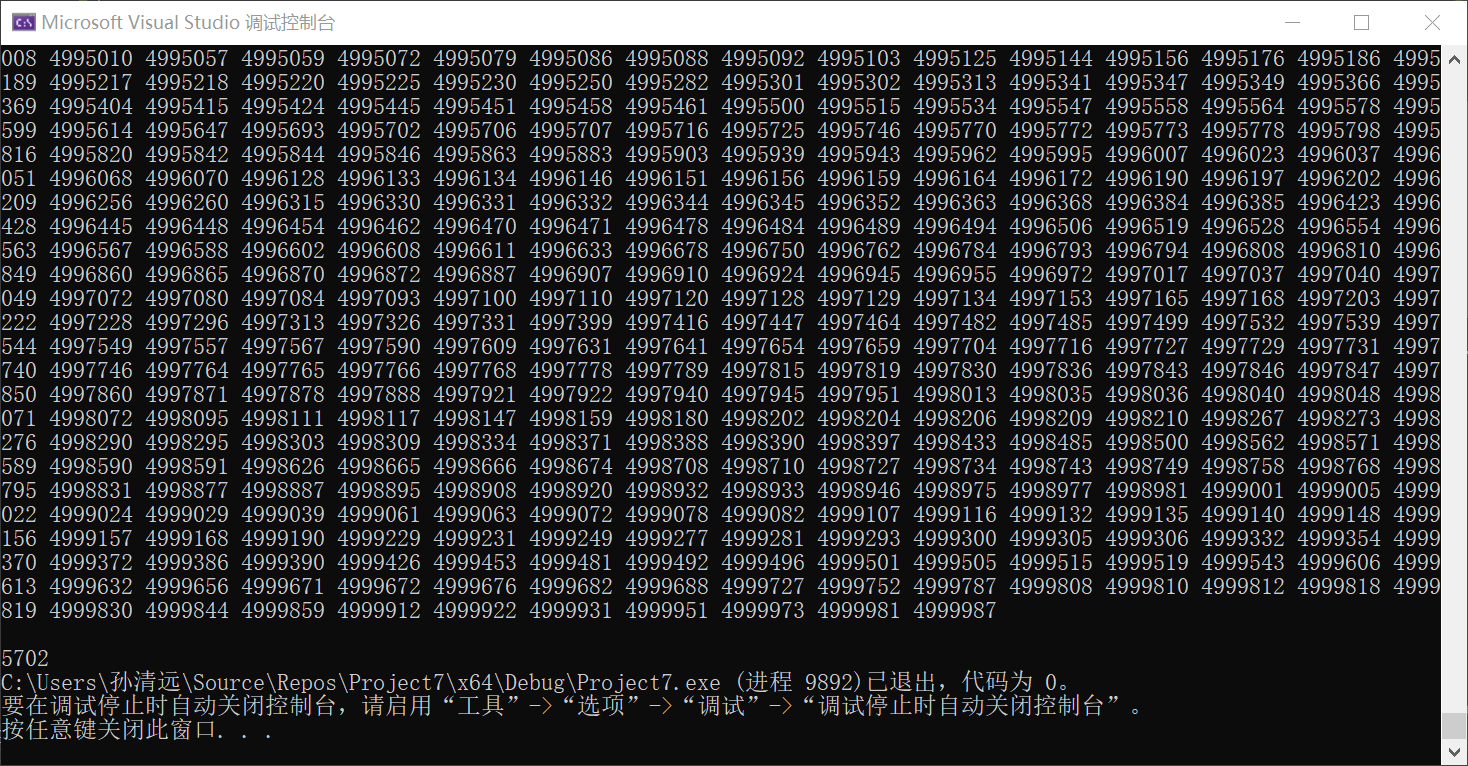
\includegraphics[width=0.9\textwidth]{quick0.png}
    \caption{QuickSort1}
\end{figure}
\begin{figure}[H]
    \centering
    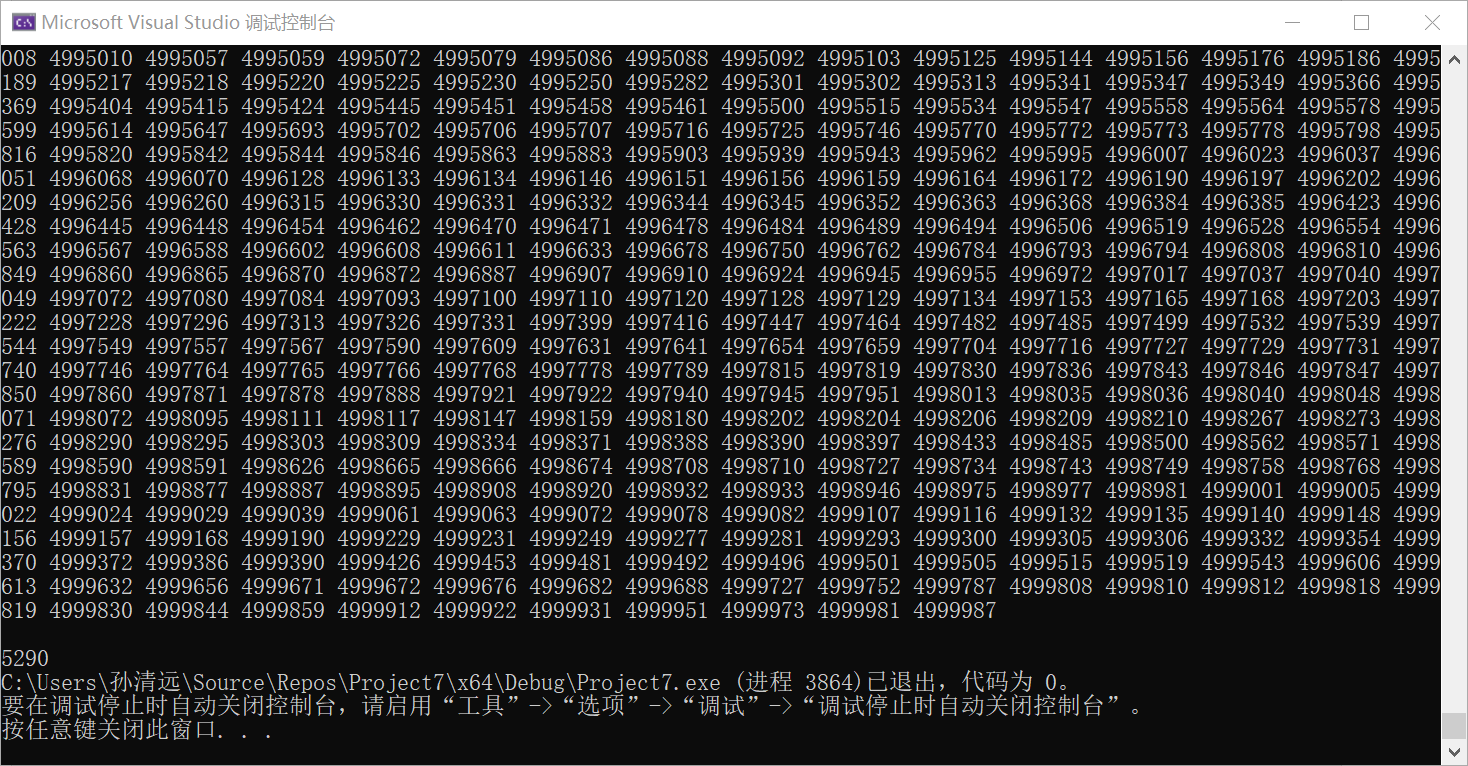
\includegraphics[width=0.9\textwidth]{quick1.png}
    \caption{QuickSort2}
\end{figure}
以上两幅图显示了采用第一与第二个数据集时,快速排序运行的结果,由于
将11个数据集的结果展示出来篇幅过长,因此采用折线图的形式进行表示。\par
\begin{figure}[H]
    \centering
    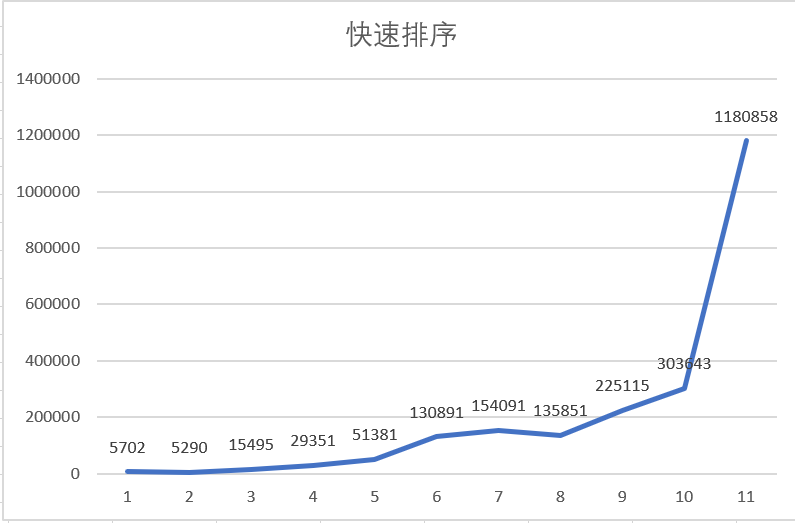
\includegraphics[width=0.7\textwidth]{figure1.png}
    \caption{执行快速排序算法随着数据集重复率的提升,\\消耗时间的变化}
\end{figure}
归并排序算法的展示如下。\par
\begin{figure}[H]
    \centering
    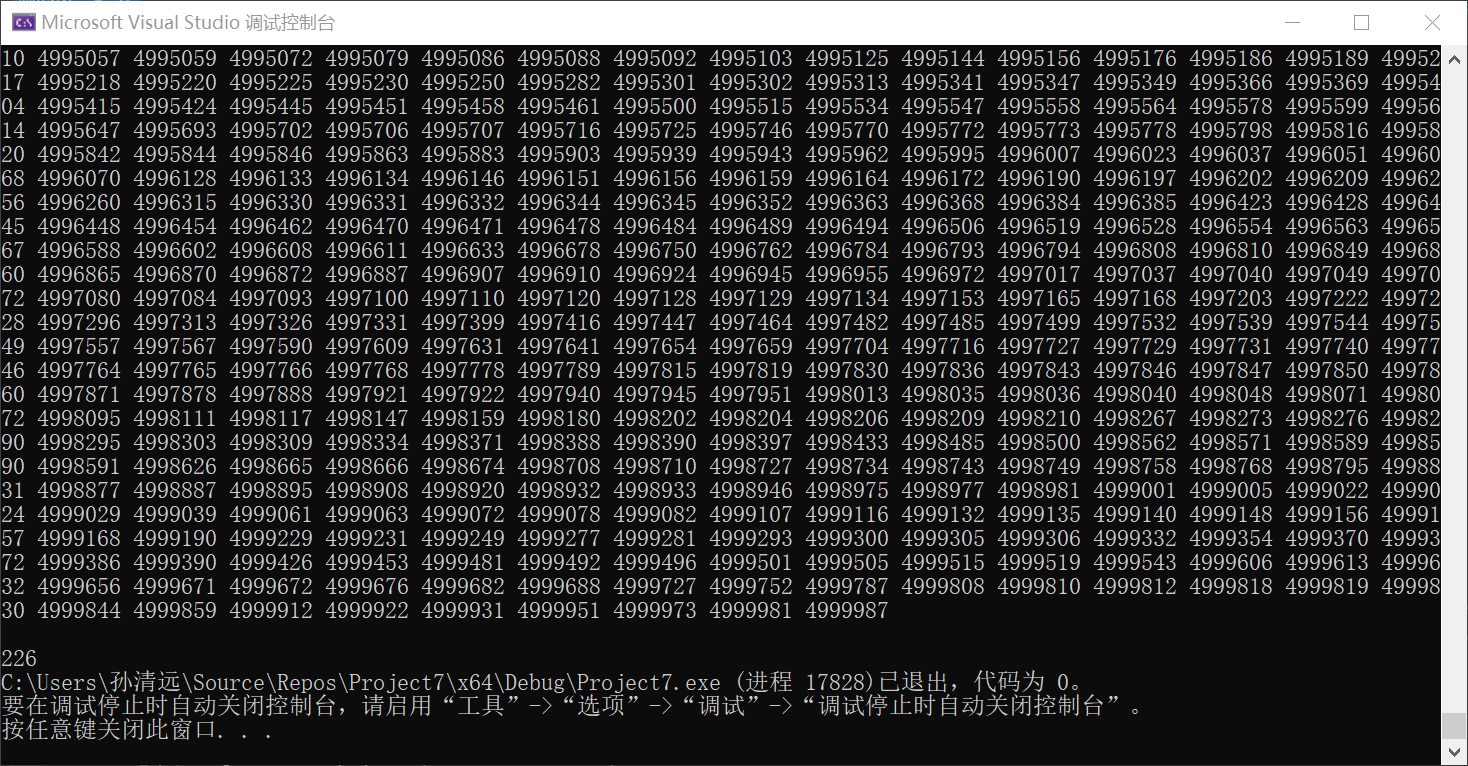
\includegraphics[width=0.9\textwidth]{merge1.png}
    \caption{MergeSort1}
\end{figure}
\begin{figure}[H]
    \centering
    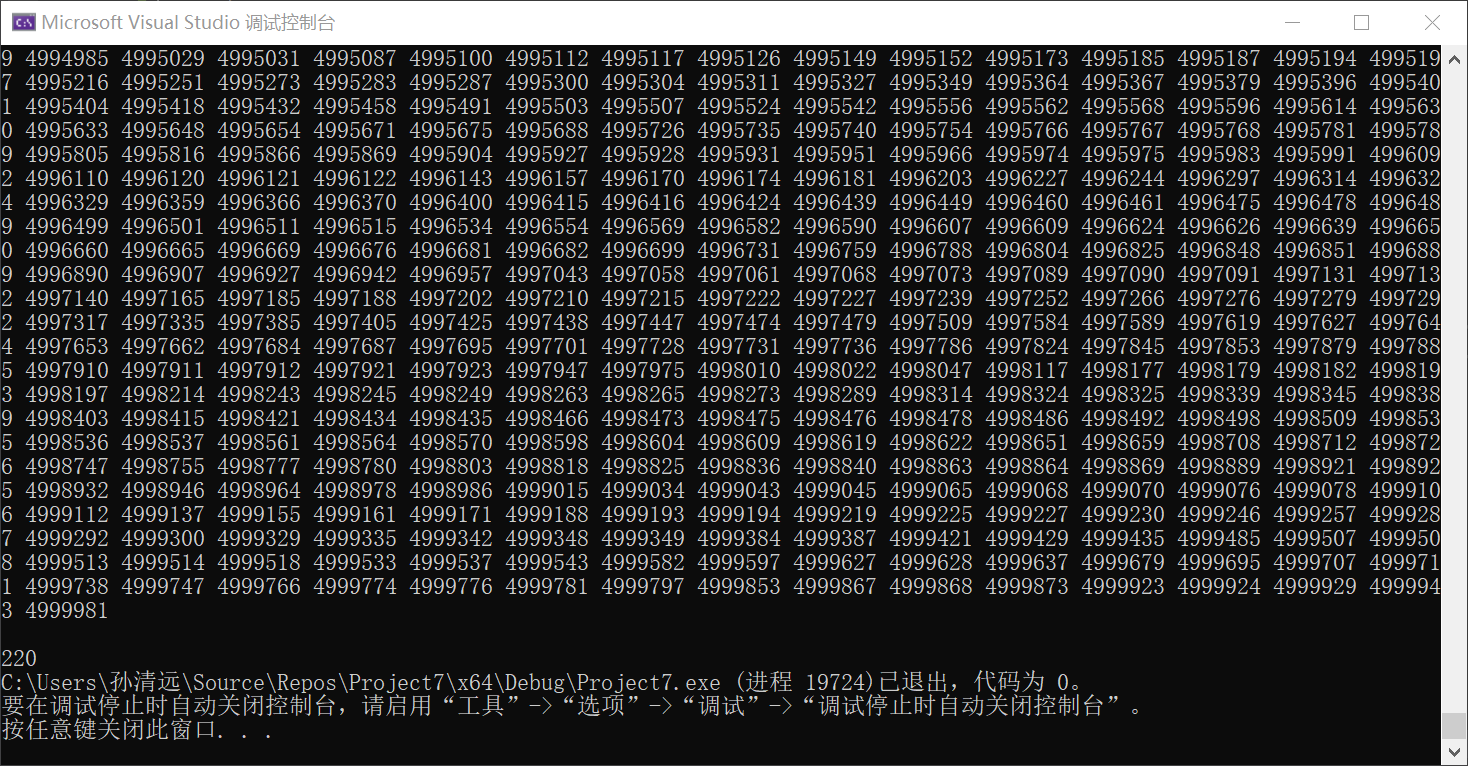
\includegraphics[width=0.9\textwidth]{merge2.png}
    \caption{MergeSort2}
\end{figure}
\begin{figure}[H]
    \centering
    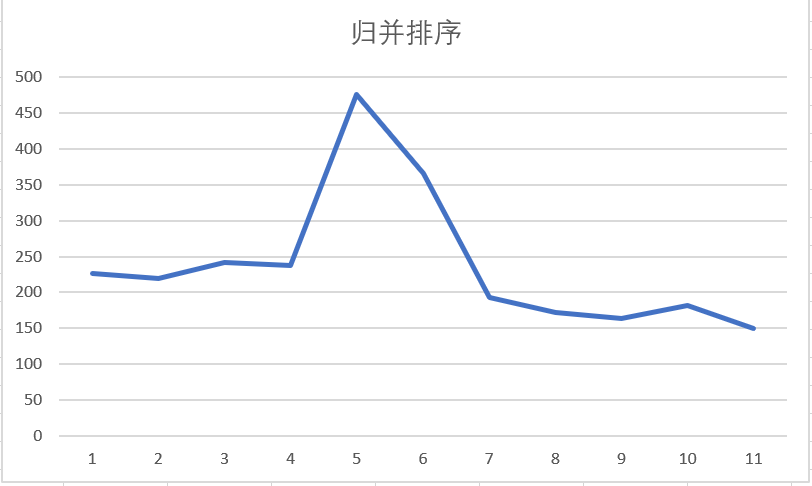
\includegraphics[width=0.7\textwidth]{figure2.png}
    \caption{执行归并排序算法随着数据集重复率的提升,\\消耗时间的变化}
\end{figure}
\subsection{结果分析}
\subsubsection{库函数执行结果}
在上述数据集上运行库函数得到的结果如下。
\begin{figure}[H]
    \centering
    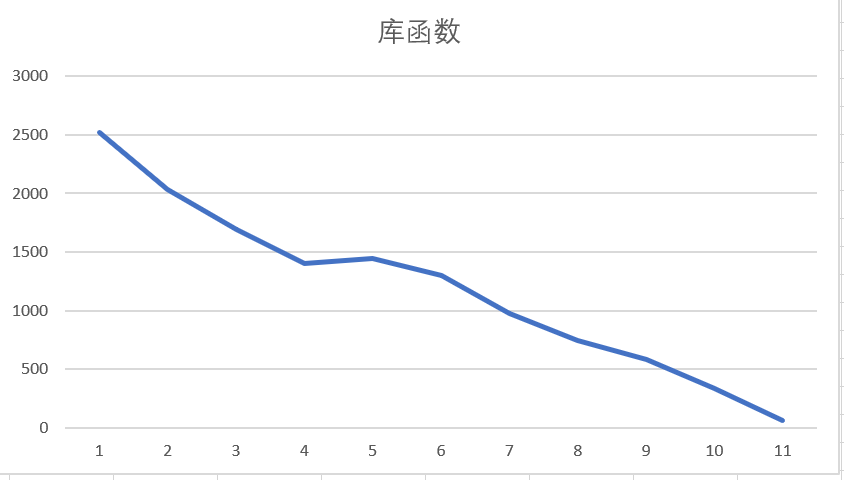
\includegraphics[width=0.7\textwidth]{figure3.png}
    \caption{执行随着数据集重复率的提升,\\消耗时间的变化}
\end{figure}
\subsubsection{结果推测与解释}
对于快速排序,由于其复杂度被基准点的选择和数据的重复率所决定,因此算法运行时间
有一定的随机性,但总体来说,随着重复率的增加,时间开销是增加的。\par
归并排序的原理说明了数据的重复率与算法时间复杂度并没有太大关系,在相同的数据规模下,
算法运行时间大致相同。\par
在执行库函数时,随着数据重复率的上升,算法的运行时间不升反降,在sort函数中,一旦数据规模超过某个值
就执行快速排序,否则执行插入排序。在快速排序实现的过程中,应该也会有专门针对重复数据的处理措施。\par
\subsubsection{改进措施}
\begin{itemize}
    \item 可根据数据规模的不同,执行不同的排序算法,以此来提升效率。
    \item 针对快速排序,增加使两个集合划分均匀的措施,例如随机选取,三点中值等。
\end{itemize}
\section{找第k小的数}
\thispagestyle{empty}
\subsection{算法原理}
实验要求实现两种基于分治策略的选第k大算法,此实验选取的两种算法如下。
\subsubsection{排序选第k小}
直接对数据集运行快速排序,然后给出第k小的数。
\subsubsection{BFPRT算法}
BFPRT算法,又称为中位数的中位数算法,由5位大牛(Blum 、 Floyd 、 Pratt 、 Rivest 、 Tarjan)提出,并以他们的名字命名。
\par
算法的思想是修改快速选择算法的主元选取方法,提高算法在最坏情况下的时间复杂度。其主要步骤为:
\begin{enumerate}
    \item 首先把数组按5个数为一组进行分组,最后不足5个的忽略。对每组数进行排序(如插入排序)求取其中位数。
    \item 把上一步的所有中位数移到数组的前面,对这些中位数递归调用BFPRT算法求得他们的中位数。
    \item 将上一步得到的中位数作为划分的主元进行整个数组的划分。
    \item 判断第k个数在划分结果的左边、右边还是恰好是划分结果本身,前两者递归处理,后者直接返回答案。
    \item base case :在某次递归调用BFPRT算法时发现这个区域只有一个数,那么这个数就是我们要找的数。
\end{enumerate}
\subsection{算法描述}
执行排序选第k小的算法伪码在实验一中已经描述过,在此不多赘述。
下面给出BFPRT算法的伪码描述。\par
算法Select(S,k)\par
输入:数组S,正整数k\par
输出:S中第k小的元素
\begin{enumerate}
    \item 将S分5个一组,共$\lceil n/5 \rceil$组
    \item 每组排序,中位数放到集合M
    \item $m^* \gets Select(M,\lceil M/2 \rceil)$//S分A,B,C,D
    \item A,D元素小于$m^*放S_1,大于m^*放S_2$
    \item $S_1 \gets S_1 \cup C; S_2 \gets S_2 \cup B$
    \item $if \ k= \mid S_1 \mid +1$ \ then 输出$m^*$
    \item else if $k \le \mid S_1 \mid$
    \item \qquad Select($S_1$,k)
    \item \qquad Select($S_2,k-\mid S_1 \mid -1$)
\end{enumerate}
\subsection{算法程序}
同样的,在此处只介绍BFPRT算法的实现。\par
\begin{lstlisting}[language=C++]
int partition(int A[], int low, int high)
{
	int pivot = A[low];
	while (low < high){
		while (low < high && A[high] >= pivot){
			--high;
		}
		A[low] = A[high];
		while (low < high && A[low] <= pivot){
			++low;
		}
		A[high] = A[low];
	}
	A[low] = pivot;
	return low;
}
int r = 5;
int Select(int A[], int low, int high, int k)
{
	int r_group = ceil((high - low + 1)*1.0 / r);
	for (int i = 1; i <= r_group; ++i) {
		sort(&A[low + (i - 1)*r], &A[(low + i*r - 1) > high ? high : (low + i*r - 1)]);
		swap(A[low + i - 1], A[low + (i-1)*r + r / 2]);
	}
	sort(&A[low], &A[low + r_group]);
	swap(A[low], A[r_group / 2]);
	int cur = partition(A, low, high);
	if (cur == k-1){
		return A[cur];
	}
	else if (cur < k){
		return Select(A, cur + 1, high, k);
	}
	else{
		return Select(A, low, cur - 1, k);
	}
}
\end{lstlisting}
\subsection{实验结果}
两种算法的平均运行时间如下。
\begin{table}[H]
    \caption{平均运行时间}
    \centering
    \begin{tabular}{p{2cm}p{2cm}p{2cm}}
\hline
数据集大小 & BFPRT算法 & 排序选第k小 \\
\hline
1000 & 2.43 & 0.12 \\
2000 & 6.57 & 0.5 \\
5000 & 14.23 & 1.27 \\
10000 & 35.29 & 2.42 \\
20000 & 69.52 & 5.63 \\
50000 & 215.81 & 13.9 \\
100000 & 403.68 & 32.32 \\
200000 & 681.42 & 75.33 \\
500000 & 1303.7 & 222.79 \\
1000000 & 2465.76 & 589.79 \\
\hline
       \end{tabular}
\end{table}
\subsection{结果分析}
由如上结果绘制出流程图。
\begin{figure}[H]
    \centering
    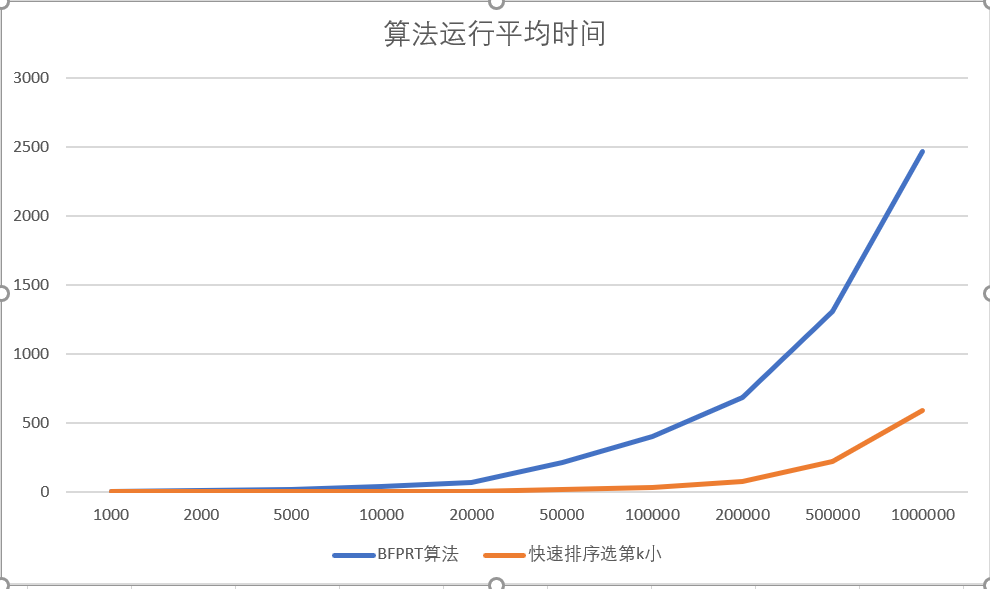
\includegraphics[width=0.8\textwidth]{figure4.png}
    \caption{算法执行时间}
\end{figure}
由上图可知,在数据量较大时,BFPRT算法表现明显优秀,而在数据量较小时,二者并无
明显区别。
\end{document}